\chapter{Merge di ontologie}
\label{ch4}
\section{Intoduzione}
In questo capitolo vediamo come sia possibile usare \cduce per fare il merge di ontologie, cercando di mettere in risalto quelli che possono essere i vantaggi di usare un linguaggio funzionale rispetto a uno strumento grafico. Alla fine del capitolo paragoneremo l'approccio con \cduce a quello con Protégé. Per mettere in evidenza i vantaggi di \cduce presentiamo un esempio un po' più complesso di quelli visti in precedenza in modo da far risaltare le potenzialità di \cduce e contemporaneamente dare un'idea di funzioni più complesse.

\section{Obiettivo del merge}\label{ch4.1}
Adesso che abbiamo creato un ontologia a partire dall'\say{European Fashion Thesaurus} e abbiamo descritto una semplice ontologia per descrivere persone, vorremmo fonderle in una nuova ontologia che possa parlare degli usi e costumi della società, magari riferita a un ben preciso periodo storico. Vogliamo creare un'ontologia in cui sia possibile rappresentare delle persone, coi rispettivi legami di parentela e nella quale sia possibile associare alle persone uno status sociale, un lavoro e uno specifico abbigliamento.
\subsection{Ontologie di partenza}
Per creare questa ontologia consideriamo 3 ontologie di partenza:

\verb|society|: è lo scheletro dell'ontologia che vogliamo ottenere: è comodo crearla a priori in modo da non dover creare ex novo tutta la struttura in \cduce, inizialmente rappresenta delle persone sulle quali definiamo le relazioni \verb|born_in|, \verb|is| e \verb|work_as| che associano una persona con la città di nascita, con il suo status sociale e con il proprio lavoro;
\begin{figure}[H]
	\centering
	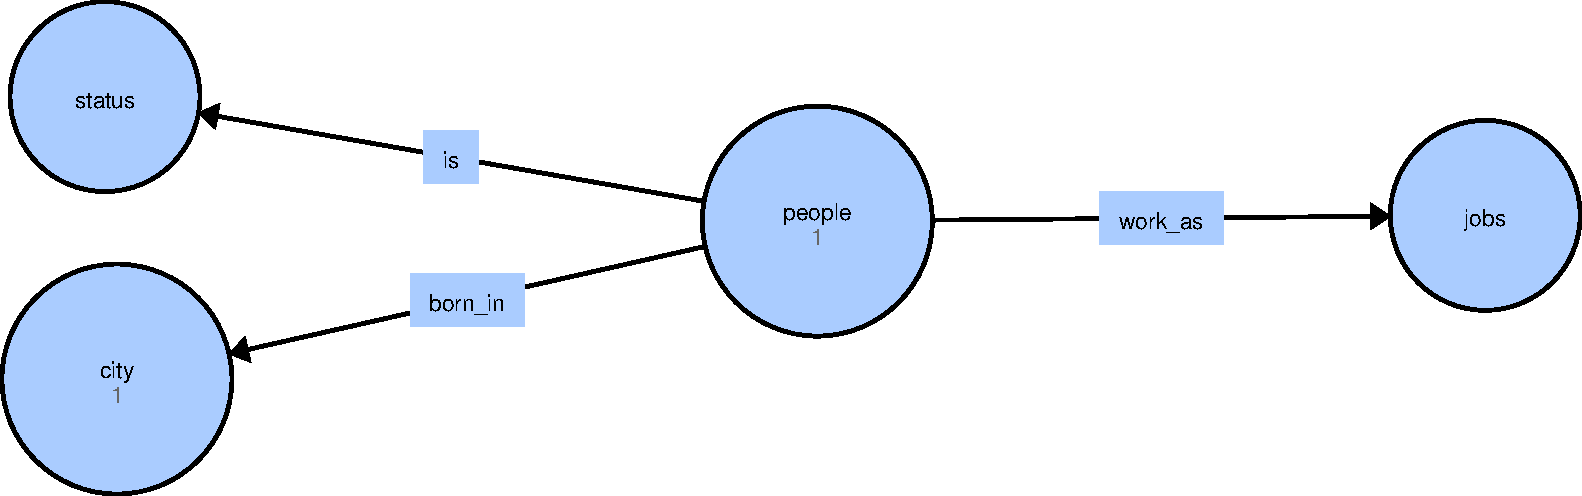
\includegraphics[width=0.5\textwidth]{Picture/society.rdf.pdf}
	\caption{grafo ontologia \texttt{society}}
\end{figure}

\verb|people|: rappresenta gli individui con le loro parentele: rispetto all'ontologia presentata in \ref{lst:persone.rdf} abbiamo aggiunto la relazione simmetrica \verb|marry|, e la relazione \verb|son_of| come inversa di \verb|parent_of|, aggiungiamo anche l'anno di nascita e morte.
\begin{figure}[H]
	\centering
	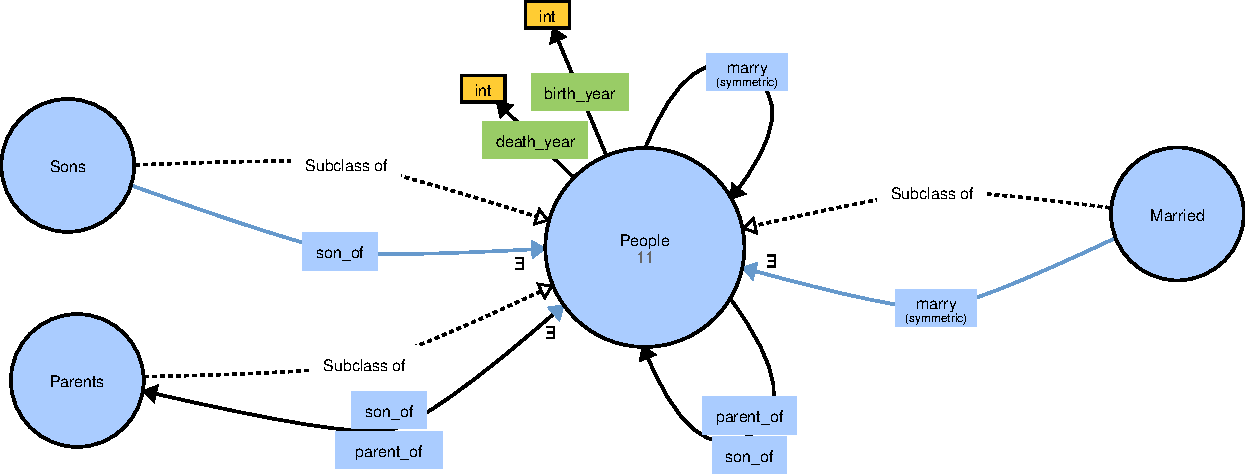
\includegraphics[width=0.5\textwidth]{Picture/people.2.pdf}
	\caption{grafo ontologia \texttt{people}}
\end{figure}

\phantomsection\label{ont_fashion}
\verb|fashion|: è l'ontologia che abbiamo creato nel capitolo \ref{ch3} arricchita con le relazioni \verb|made_of|, \verb|crafted_with|, \verb|color|, che indicano rispettivamente i materiali costituenti, le tecniche realizzative e i colori di un capo d'abbigliamento. Anche di questa ontologia presentiamo il grafo, l'ontologia ha moltissime classi, per non creare un grafo inutilmente complesso lo tagliamo a una certa profondità\footnote{Dall'immagine sembrano esserci classi orfane o fibre che non sono sottoclasse di materiali, questa è un'imprecisione dovuta al fatto che WebVOWL non lavora esattamente tagliando il grafo a una certa profondità, ma collassa molte classi in una singola, questo produce effetti indesiderati. Se si rappresentasse l'ontologia con tutte le classi si apprezzerebbe la struttura corretta, ma il grafo sarebbe illeggibile}. Per rendere ulteriormente più chiara l'immagine abbiamo colorato in rosso le classi principali (oggetti di moda, colori e materiali). 
\label{fig_eur}
\begin{figure}[H]
	\centering	
	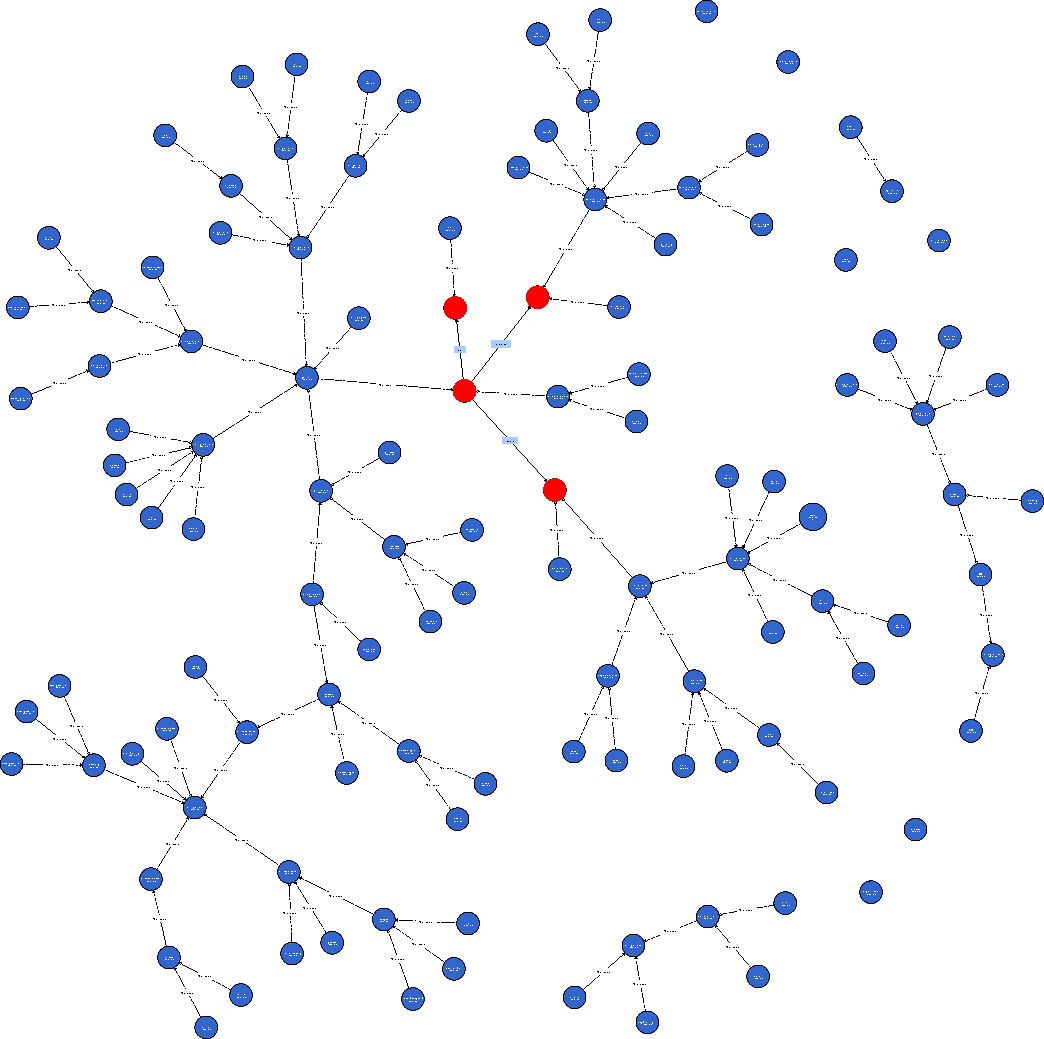
\includegraphics[width=0.5\textwidth]{Picture/europeana_formatted.rdf.pdf}
	\caption{grafo ontologia \texttt{europeana}}
\end{figure}
\subsection{Ontologia di arrivo}
Vogliamo modificare \verb|society| in modo da descrivere gli usi e i costumi della società del XII secolo, per fare questo estrapoliamo dall'ontologia \verb|fashion| tutti i vestiti che non siano costituiti da fibre naturali e scremiamo dall'ontologia \verb|people| tutte le persone che sono vissute in un'epoca che non ci interessa. Vogliamo poi che la classe \verb|People| definita in \verb|society| sia equivalente alla classe \verb|People| definita in \verb|people|, senza perdere tutte le relazioni di parentela, e potendo contemporaneamente sfruttare le nuove relazioni definite in \verb|society|.
\section{Struttura generica di un'ontologia}
Per fare il merge dobbiamo poter caricare le 3 ontologie in \cduce, quindi descriviamo una struttura generale per fare il parsing di un'ontologia generica:
\addocaml{general structure}{lst:general_structure}{Code/general_structure.cd}
Rispetto alle strutture definite in precedenza notiamo varie aggiunte:
\begin{itemize}
	\item si specifica meglio l'elemento \verb|EqClass|: questo infatti può essere una restrizione (un genitore è una persona con dei figli) oppure un'equivalenza senza condizioni (ci serve per rendere uguali i concetti di persona definiti nelle 2 ontologie);
	\item definiamo il tipo \verb|DataProperty|: questo rappresenta una proprietà degli individui, nel nostro caso la usiamo per specificare l'anno di nascita di una persona. Gli individui nella loro lista di attributi potranno ora averne uno di tipo \verb|DataProp|;
	\item il tipo \verb|AnnProperty| serve perché avendo editato l'ontologia \verb|fashion| in Protégé (per aggiungere le relazioni non presenti nel tesauro) i tag SKOS sono stati correttamente riconosciuti \cite{OWL&SKOS} e classificati come tag \verb|owl:AnnotationProperty|;
\end{itemize}
\section{Merge}
\subsection{Funzioni utili}
Prima di passare alla costruzione della nuova ontologia vediamo alcune funzioni utili che si possono applicare a qualsiasi ontologia e che sono servite per costruire le funzioni specifiche adatte a manipolare le particolari ontologie di interesse.
\addocaml{usefull function}{lst:utility.cd}{Code/utility.cd}
Per la prima volta abbiamo fatto ricorso ad applicazioni parziali, questo è utile per poter parametrizzare anche l'ontologia di riferimento; dato che in questo caso ne manipoliamo contemporaneamente tre, è importante poter specificare volta per volta a quale ci riferiamo.

Vediamo per la prima volta degli esempi di funzioni ricorsive:
\begin{itemize}
	\item \verb|andList| e \verb|orList| (linee 22 e 26) lavorano su liste di booleani e restituiscono il risultato della congiunzione o disgiunzione logica tra tutti gli elementi di una lista. Per ottenere questo risultato si fa il pattern matching della lista che può essere un elemento in testa alla lista seguito da una lista che chiamiamo coda; la funzione restituisce l'operazione logica tra la testa e la chiamata ricorsiva alla funzione, passando come parametro la coda della lista. Quando la lista è vuota (seconda clausola del matching) la funzione restituisce l'elemento neutro dell'operazione logica;
	\item \verb|subClassRec| richiama ricorsivamente se stessa per costruire l'intero albero di sottoclassi a partire da una classe data (e dall'ontologia di riferimento). Ovviamente perché questa funzione possa terminare, la struttura delle classi deve essere un grafo aciclico (questa non è una grossa limitazione, infatti se la classe \verb|c2| è contemporaneamente sopraclasse e sottoclasse di \verb|c1|, allora \verb|c1| e \verb|c2| sono equivalenti e possono essere accorpate per eliminare i cicli, discorso analogo vale per cicli più lunghi).
\end{itemize}

Per verificare se un individuo si trova in un certo albero di classi, si potrebbe operare al contrario rispetto a \verb|subClassRec|, risalendo l'albero fino a quando non si trova il padre desiderato (restituendo \verb|true|) oppure la radice delle classi (restituendo \verb|false|). Questo approccio, però, presenta delle problematiche:
\begin{itemize}
	\item un individuo può appartenere a più classi, quindi bisognerebbe risalire \emph{n} alberi dove \emph{n} è il numero di classi a cui appartiene l'oggetto;
	\item ogni classe può essere sottoclasse di più classi diramando così ulteriormente la ricerca.
\end{itemize}
Facendo alcuni test, si nota che un approccio di questo genere, oltre a essere impegnativo dal punto di vista implementativo è anche poco efficiente dal punto di vista prestazionale. Come vedremo in \ref{lst:is_artificial.cd} per ogni capo d'abbigliamento dovremo chiederci se è costituito da materiali artificiali e questo rallenta il processo di merge. Per evitare questo problema costruiamo solo una volta la lista di materiali artificiali e, quando dobbiamo stabilire se un materiale è naturale o meno, verifichiamo se appartiene alla lista dei materiali artificiali. Questo approccio è vantaggioso in quanto la lista di materiali artificiali andrebbe creata in ogni caso per andare ad aggiungere alla nuova ontologia tutti i materiali che non lo sono (conviene creare la lista dei materiali artificiali piuttosto che quella dei materiali naturali perché la prima contiene molti meno elementi, di conseguenza è più veloce da creare).

Per implementare questa ricerca usiamo \verb|isInClasses| (linea 46) che prende un individuo e una lista di classi, valuta a che classi appartiene l'individuo (con \verb|classOf|) e usa la funzione \verb|contains| per creare una lista di valori booleani uno per ogni classe dell'individuo, verificando se è contenuto nella lista di classi fornita; infine si verifica se la lista di booleani contiene solo \verb|true| con la funzione \verb|andList|

\subsection{Selezione degli abiti}
Mostriamo come si possano importare solo le fibre naturali e i vestiti costituiti esclusivamente da questi materiali, questo ha lo scopo di presentare come si possa fare della semplice inferenza sulla base di conoscenza usando solamente \cduce e senza ricorrere a reasoner esterni più sofisticati e complessi. Non mostriamo le funzioni per selezionare solo le persone vissute nel periodo storico considerato, questo per non inserire troppo codice e perché sarebbe poco istruttivo (non introdurremmo nuovi concetti rispetto a quelli che presentiamo in seguito).

Per ragionare sul singolo abito ci domandiamo di che materiali è fatto usando la relazione \verb|made_of| che associa uno o più materiali a un abito. Una volta che abbiamo i materiali, possiamo considerare la struttura ad albero dei materiali dell'ontologia \verb|fashion| (la struttura è quella importata dal tesauro \say{European Fashion Thesaurus}) per distinguere materiali naturali da artificiali (le due categorie devono essere disgiunte). Un vestito verrà considerato valido per la nuova ontologia solo se costituito unicamente da fibre naturali\footnote{Possiamo fare inferenza solo con i dati in nostro possesso, in particolare la classe dei materiali si divide in tre sottoclassi che rappresentano materiali naturali, artificiali e materiali di decorazione; su questi ultimi non possiamo fare alcun ragionamento sull'origine, si è operata una scelta permissiva considerandoli tutti naturali}.

Una possibile implementazione delle funzioni che ci permettono di stabilire se un abito è costituito esclusivamente da fibre naturali è la seguente:
\addocaml{test artificial}{lst:is_artificial.cd}{Code/is_artificial.cd}
La funzione \verb|madeOf| restituisce una lista di individui che sono tutti i materiali di cui è costituito un abito, per fare questo \verb|madeOf| prende come parametri l'abito e l'ontologia di riferimento. 

La funzione \verb|isArtificial| ha 2 comportamenti differenti a seconda dell'individuo che le viene passato come parametro:
\begin{itemize}
	\item materiale: se l'individuo appartiene all'albero dei materiali, il controllo consiste nello stabilire se questo materiale appartiene alla lista dei materiali artificiali: se è così si restituisce \verb|true|
	\item indumento: se l'individuo appartiene a una sottoclasse dei vestiti, prima si crea la lista di materiali di cui è costituito, poi si valuta: se almeno uno di questi è artificiale si restituisce \verb|true|
\end{itemize}
Per poter fare queste operazioni la funzione riceve come parametri: l'individuo da analizzare, la lista di tutti i materiali, la lista dei materiali artificiali e  l'ontologia di riferimento.
\subsection{Costruzione dell'ontologia}
Assembliamo tutti i pezzi visti finora per manipolare l'ontologia \verb|society| aggiungendo tutte le classi e gli individui che ci interessano. Presentiamo subito l'implementazione descrivendola poi passo passo.
\addocaml{assemble ontology}{lst:make_ontology.cd}{Code/make_ontology.cd}
Da riga 1 a riga 3 carichiamo le ontologie che useremo, poi andiamo a creare le liste di classi di materiali che ci servono per utilizzare le funzioni definite in \ref{lst:utility.cd} e \ref{lst:is_artificial.cd}: tutti i materiali e materiali artificiali. Creiamo anche la lista di tutte le classi di vestiti.

Alla riga 9 costruiamo la lista di classi dei materiali ammissibili per la nuova ontologia selezionando dalla lista totale tutti quelli non artificiali. In riga 12 estraiamo tutti i vestiti (individui) costituiti solo da materiali naturali (nella nuova ontologia inseriamo tutte le classi di vestiti, queste possono potenzialmente rappresentare individui fatti di fibre naturali).

Alla riga 17 prendiamo tutti gli elementi dell'ontologia \verb|society| escluso l'elemento di tipo \verb|Ont| e la classe \verb|people|, questo perché l'elemento \verb|Ont| verrà ricreato da zero alla riga 24 e la classe \verb|people| andrà modificata per renderla equivalente alla classe \verb|people| dell'ontologia \verb|people| (riga 20)

In questo esempio prendiamo tutti gli elementi dell'ontologia \verb|people|; come detto prima, presentare il codice per selezionare solo alcune persone sarebbe poco istruttivo. Una volta create tutte le nuove liste di elementi, le assembliamo alla riga 26 e, alla riga 28 costruiamo la nuova ontologia; in riga 30 la salviamo su file.
\subsection{Risultato finale}
L'ontologia che abbiamo costruito permette di descrivere la società nelle modalità che ci eravamo prefissati all'inizio del capitolo (\ref{ch4.1}), inoltre abbiamo importato già tutte le persone che avevamo modellato nell'ontologia \verb|people| mantenendo le loro relazioni di parentela; possiamo definire nuove relazioni di parentela sulle persone già modellate in \verb|society| (oppure attribuire loro una data di nascita) e usare le relazioni definite in \verb|society| per arricchire la descrizione di un individuo presente in \verb|people|. Abbiamo anche importato tutte le classi di vestiti e tutti i materiali naturali dall'ontologia \verb|fashion|, possiamo ora creare nuove relazioni tra persone e vestiario  per aggiungere informazioni sugli usi e costumi della società che intendiamo descrivere.

Del risultato finale riportiamo solo la parte di grafo che descrive le persone, la parte che descrive il vestiario è esattamente uguale a quella riportata in \ref{fig_eur} alla quale togliamo le fibre artificiali. Il grafo che descrive le persone ci fa apprezzare come effettivamente le due classi estratte, una dall'ontologia \verb|society| e l'altra dall'ontologia \verb|people|, siano effettivamente state accorpate\footnote{In realtà rimangono due classi ma sono dichiarate equivalenti} in un unica classe che possiede tutti gli attributi e le relazioni delle due classi di partenza.
\begin{figure}[H]
	\centering
	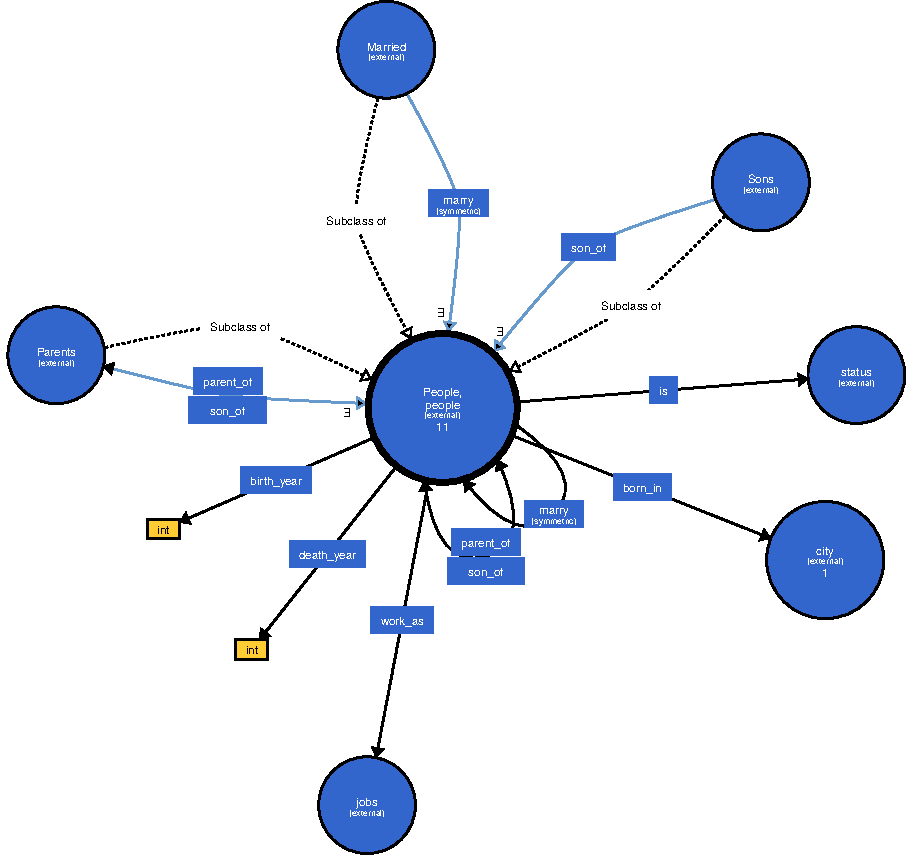
\includegraphics[width=0.5\textwidth]{Picture/society_merged.rdf.pdf}
	\caption{grafo ontologia \texttt{society merged}}
\end{figure}

\section{In Protégé}
In Protégé esiste un comando per fare il merge di ontologie: una volta aperte tutte le ontologie che siamo interessati a fondere, possiamo farne il merge e Protégé si occupa di creare una nuova ontologia e inserire tutte le classi, gli individui, le relazioni e le proprietà di tutte le ontologie di partenza. 

Questo approccio è molto comodo se siamo interessati a prendere tutti i concetti dalle ontologie di partenza, in questo caso l'unico lavoro che ci rimane da fare è quello di mettere in relazione corretta le classi (in questo caso rendere equivalenti le due classi che descrivono le persone). 

Nel caso in cui volessimo fare una selezione più fine su quali concetti importare dovremmo modificare le ontologie di partenza costruendo e scegliendo a prescindere (mediante delle Query) le classi e gli individui che vogliamo importare oppure, una volta fatto il merge, rimuovendo ciò che non ci interessa.
\section{Conclusioni}
Il merge con \cduce richiede di scrivere funzioni che permettano di selezionare cosa importare, questa precisione nella selezione comporta, però, più responsabilità da parte del programmatore che deve fare in modo che i dati continuino a essere consistenti e che le informazioni non vengano alterate durante il merge. Nuovamente sfruttiamo il controllo statico dei tipi offerto da \cduce: in questo caso possiamo notare che man mano che creiamo la nuova ontologia in \ref{lst:make_ontology.cd} verifichiamo che ogni elemento abbia effettivamente il tipo che ci aspettiamo. Controllando il tipo in fase di costruzione siamo sicuri che il documento che salviamo alla fine sia effettivamente un'ontologia e aprendola con un altro strumento (Protégé ad esempio) verrà riconosciuta correttamente e non ci saranno inconsistenze.

Nel caso specifico, il controllo di tipo è stato importante, infatti, la modifica della classe \verb|socPeople| (riga 20 in \ref{lst:make_ontology.cd}) non era andata a buon fine e aveva generato un elemento XML che non faceva più il match con l'elemento di tipo \verb|Class| definito in \ref{lst:general_structure}. Avremmo comunque potuto salvare il risultato, ma se avessimo tentato di trattarlo come un file che descrive un'ontologia aprendolo con un altro software, avremmo ottenuto un messaggio d'errore (come se il file fosse corrotto) perché il programma non sarebbe stato in grado di interpretare il file come un file \verb|.rdf| ben formato che descrive un'ontologia.


Il merge con Protégé, per quanto lineare, richiede comunque di formulare delle Query più o meno raffinate oppure di eliminare tutto ciò che non serve agli obbiettivi del merge, il processo quindi non è molto più guidato o automatico rispetto alla controparte in \cduce. Come si può vedere dal codice in \ref{lst:utility.cd} e \ref{lst:is_artificial.cd} la maggior parte del lavoro consiste nel creare funzioni che permettano di selezionare cosa importare, una volta fatto questo il codice in \ref{lst:make_ontology.cd} che assembla l'ontologia risulta quasi banale. Selezionare elementi con funzioni in \cduce oppure con query in protégé richiede, in entrambi i casi, un certo impegno a livello di programmazione; considerando inoltre che in Protégé una volta selezionati gli elementi con delle Query è comunque necessario eliminare tutti gli altri, \cduce si rivela più efficace potendo importare esattamente ciò che si vuole (a patto di poterlo selezionare).

In conclusione Protégé è uno strumento vantaggioso nei casi in cui si voglia fare il merge tra ontologie mantenendo tutti i concetti rappresentati dalle ontologie di partenza, inoltre manipolando le informazioni con delle Query in Protégé siamo sicuri di ottenere delle ontologie consistenti. Quando è importante selezionare finemente i dati da importare, \cduce si rivela lo strumento migliore, avendo capacità espressiva e manipolativa superiore al set di strumenti base di Protégé (anche in questo caso non prendiamo in considerazione i plug-in che permettono di sviluppare programmi java per manipolare l'ontologia in Protégé). Con il controllo di tipi, \cduce fornisce comunque un certo supporto per verificare che le manipolazioni sulle ontologie portino a strutture consistenti.